%
% CURVAS ELÍPTICAS
%
\section{Curvas Elípticas}

\subsection{Definição}
``Curvas elípticas não são elipses. Elas têm esse porque são descritas por equações cúbicas, semelhantes às usadas para calcular a circunferência de uma elipse'' \cite{Stallings:2011}. Uma curva elíptica $E$ definida sobre um corpo $K$ é descrita pela equação:
\begin{equation}
y^2 + axy + by = x^3 + cx^2 + dx + e \label{eq:5}
\end{equation}
onde \(a, b, c, d\) e \(e\) são elementos do corpo $K$ e \(x\) e \(y\) são as variáveis da equação e assumem valores dentro de $K$. A notação utilizada para indicar que uma curva elíptica $E$ está definida sobre um corpo $K$ é $E/K$ e o corpo $K$ é chamado de corpo subjacente da curva \cite{Guide}. Equações deste tipo são conhecidas como \textit{equações de Weiestrass}. Com frequência, no estudo de criptografia de curvas elípticas, é costume utilizar-se a forma reduzida de Weiestrass, descrita pela equação abaixo, obtida através de uma mudança de variáveis.
\begin{equation}
y^2 = x^3 + ax + b \label{eq:6}
\end{equation}

É imprescindível que os valores de $a$ e $b$ sejam escolhidos tais que $4a^3 + 27b^2 \ne 0$ \cite{Mandy:2007}. Essa condição garante que não existe ponto na curva que possua mais de uma reta tangente \cite{Guide}.

O conjunto dos pontos que pertencem à curva elíptica $E$ definida sobre um corpo $K$ é descrito por:

$$ E(F) = \{(x,y) \in F \times F \mid y^2 = x^3 + ax + b\} \cup \{\mathcal{O}\} $$
onde o ponto $\mathcal{O}$ é chamado de \textit{ponto no infinito}. \cite{Mandy:2007}.
Será visto na próxima seção que, juntamente com uma operação de soma dos pontos da curva elíptica, o conjunto $E(F)$ forma um grupo abeliano com o ponto no infinito sendo o elemento identidade \cite{Guide}.

A Figura \ref{fig:curvas} apresenta alguns exemplos de curvas elípticas usando a forma normal da equação de Weierestrass.(OBS: CITAR A FONTE DA IMAGEM)

\begin{figure}[h]
\centering
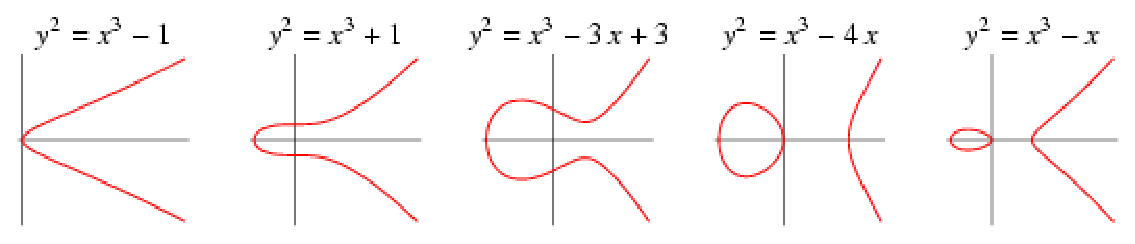
\includegraphics[scale=0.5, bb=0 0 529 101]{figuras/curvas.eps}
\caption{Exemplos de curvas elípticas}
\label{fig:curvas}
\end{figure}

\subsection{Leis de grupo para Curvas Elípticas}

Seja o conjunto de pontos $E(K)$ da curva elíptica $E$ definida sobre um corpo $K$, é possível definir uma operação sobre esse conjunto de pontos, que será chamada de adição e indicada por $+$. Essa operação de adição e o conjunto de pontos $E(K)$ da curva elíptica formam um grupo abeliano \cite{Stallings:2011}.

A forma mais clara de entender a operação de adição sobre curvas elípticas é geometricamente (ver figura \ref{fig:pontos}). A citação abaixo descreve como somar dois pontos da curva elíptica.
\begin{citacao}
Para somar dois pontos \(P\) e \(Q\) com coordenadas \(x\) diferentes, desenhe uma linha reta entre eles e encontre o terceiro ponto de interseção \(R\). Pode-se ver facilmente que existe um único ponto \(R\) que é o ponto de interseção (a menos que a linha seja tangente à curva em \(P\) ou \(Q\), quanto consideramos $R=P$ ou $R=Q$, respectivamente). Para formar uma estrutura de grupo, precisamos definir a adição sobre três pontos da seguinte forma: $P+Q=-R$. Ou seja, definimos $P+Q$ como sendo a imagem-espelho (com relação ao eixo \(x\)) do terceiro ponto da interseção. \cite{Stallings:2011} (Pg ???)
\end{citacao}

Se as coordenadas $x$ dos pontos $P$ e $Q$ são iguais, então a reta que passa pelos dois pontos não intersecta a curva elíptica em nenhum outro ponto. Para definir a estrutura de grupo, considera-se que essa reta vertical intersecta a curva no ponto no infinito $\mathcal{O}$. \cite{Stallings:2011}

É possível calcular o dobro de um ponto $P$, ou seja, calcular a soma do ponto com ele mesmo. Para isso desenha-se a reta tangente à curva no ponto $P$. Essa linha intersecta a curva elíptica num segundo ponto, que será refletido para obter-se o ponto $R$, que é o resultado da soma. \cite{Guide}

\begin{figure}[h]
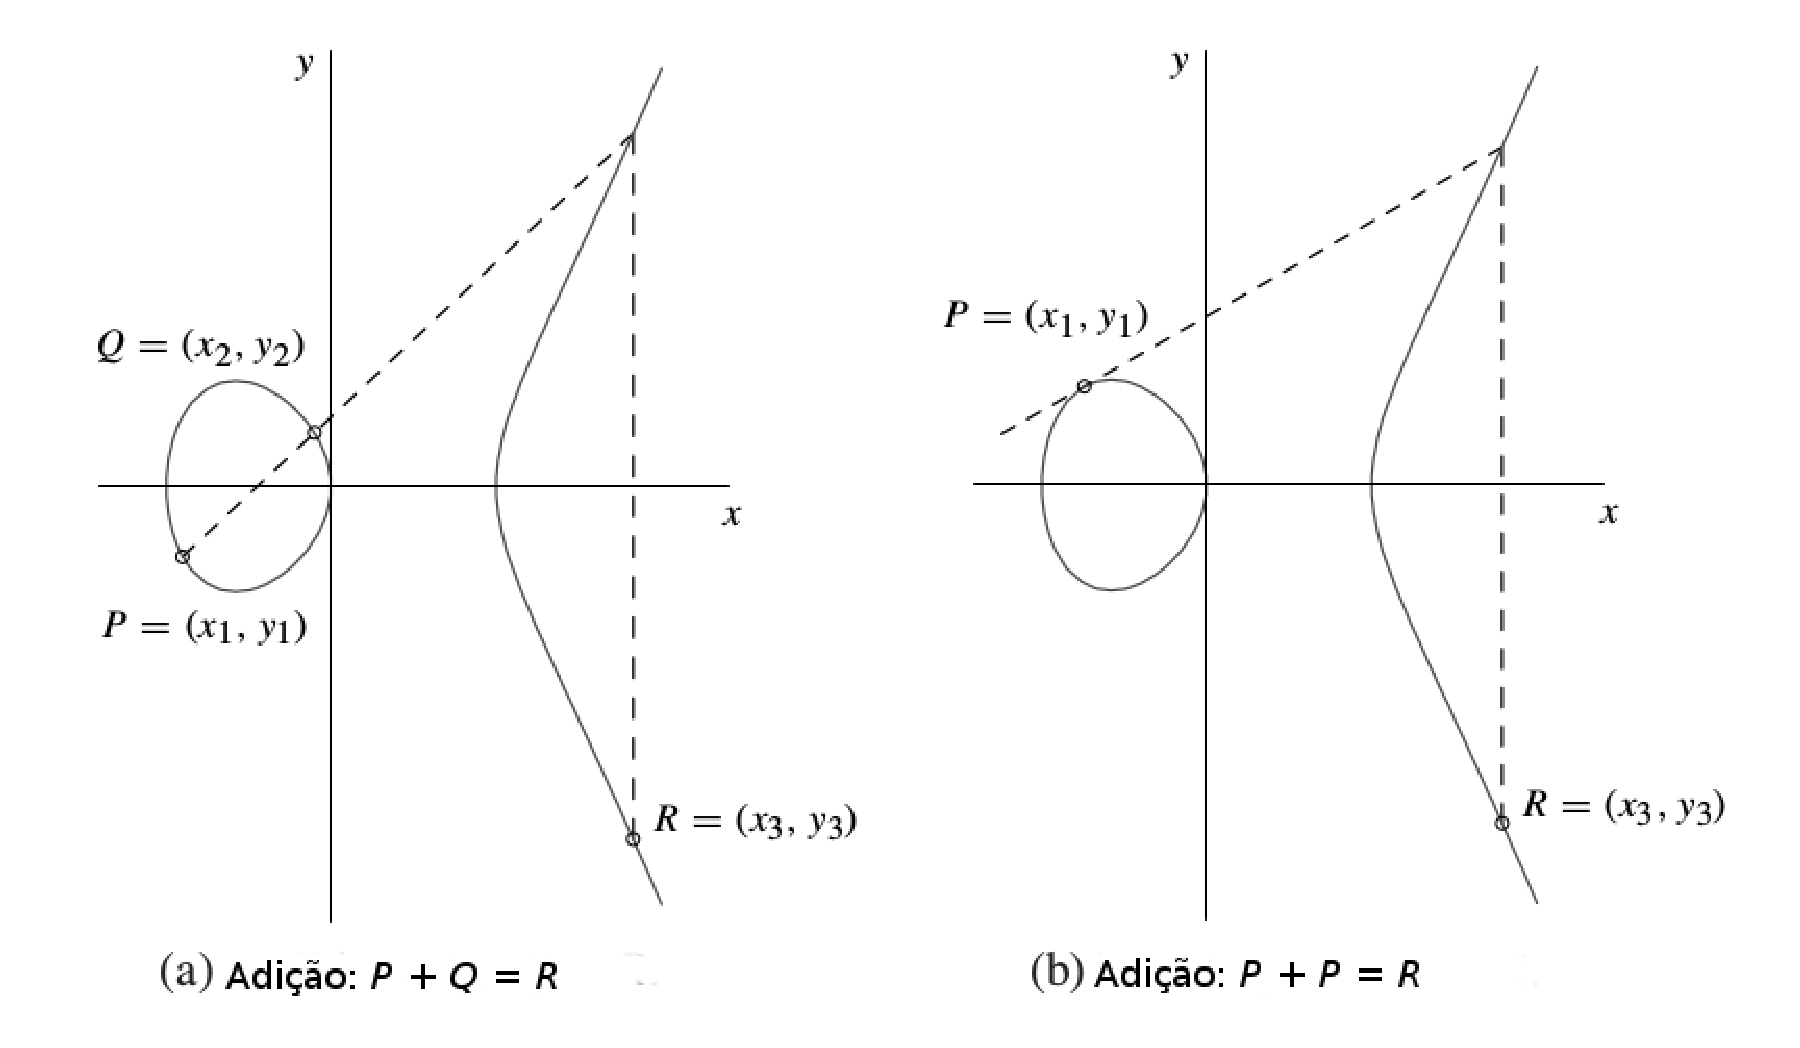
\includegraphics[scale=0.5, bb=0 0 484 636]{figuras/SomaECC.eps}
\caption{Soma de pontos em curvas elípticas \cite{Guide}}
\label{fig:pontos}
\end{figure}

Os axiomas de grupo são satisfeitos da seguinte forma:
\begin{enumerate}
  \item Para quaisquer pontos $P, Q \in E(K)$, o ponto $P + Q \in E(K)$.
  \item $\mathcal{O}$ é o elemento identidade. Logo, $P + \mathcal{O} = P$ para todo $P \in E(K)$.
  \item Para qualquer ponto $P$, existe um ponto $P'$ tal que $P + P' = \mathcal{O}$. O ponto $P'$ é denominado \textit{inverso aditivo} de $P$.
  \item A adição é associativa. Logo, $P, Q, R \in E(K)$, observa-se que $(P + Q) + R = P + (Q + R)$
  \item A adição é comutativa. Logo, $P, Q \in E(K)$, observa-se que $P + Q = Q + P$.
\end{enumerate}

\subsection{Curvas elípticas sobre corpo finito}
A criptografia de curva elíptica utiliza curvas elípticas em que as variáveis e coeficientes são todos restritos a elementos de um corpo finito, ou seja, assumem valores no conjunto de inteiros de 0 até $p - 1$ em que os cálculos são realizados módulo \(p\). Desta forma, é dito que a curva está sobre $\mathbb{F}_p$. \cite{Stallings:2011}

\begin{equation}
y^2 \mod p = (x^3 + ax + b) \mod p
\end{equation}

Pode-se mostrar que um grupo abeliano finito é definido com base no conjunto $E_p(a, b)$, desde que $(x^3 + ax + b) \mod p$ não tenha fatores repetidos. Isso é equivalente à condição

\begin{equation}
(4a^3 + 27b^2) \mod p \neq 0 \label{eq:13}
\end{equation}

A Equação \ref{eq:13} tem a mesma forma da Equação \ref{eq:7}. As regras para adição sobre $E_p(a, b)$ correspondem à técnica algébrica descrita para as curvas elípticas definidas sobre números reais. Para todos os pontos $P, Q \in E_p(a, b)$.

\begin{figure}[h]
\centering
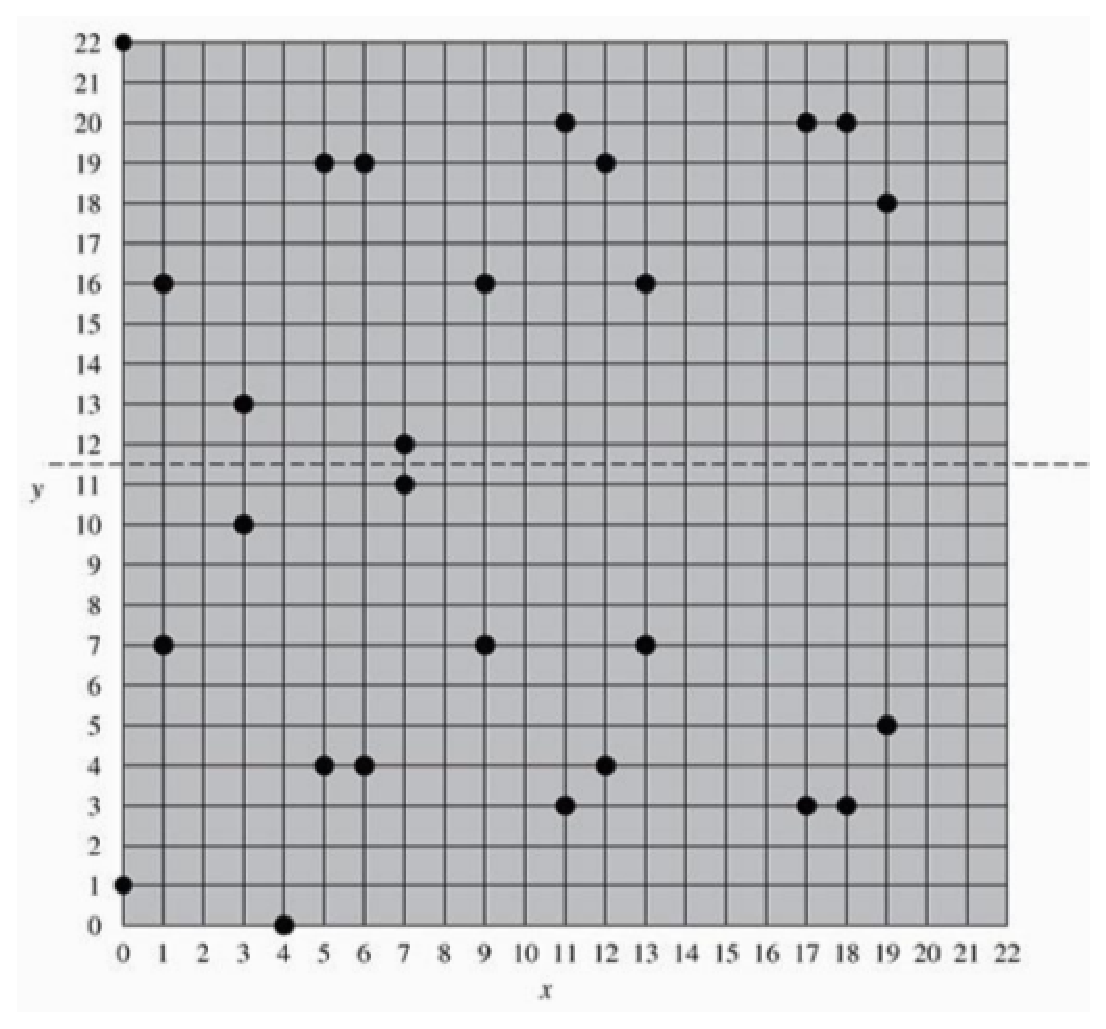
\includegraphics[scale=0.6, bb=0 0 515 478]{figuras/curva_sobre_corpo_finito.eps}
\caption{Curva elíptica $E_{23}(1, 1)$}
\label{fig:curvas}
\end{figure}

\begin{enumerate}
  \item $P + \mathcal{O} = P$.
  \item Se $P = (x_P, y_P)$, então $P + (x_P, -y_P) = \mathcal{O}$. O ponto $(x_P, -y_P)$ é o negativo de \(P\), indicado como \(-P\).
  \item Se $P = (x_P, y_P)$ e $Q = (x_Q, y_Q)$ com $P \neq -Q$, então $R = P + Q = (x_R, y_R)$ é determinado pelas seguintes regras:
    \begin{eqnarray*}
    x_R &=& (\lambda^2 - x_P - x_Q) \mod p \\
    y_R &=& (\lambda(x_P - x_R) - y_P) \mod p
    \end{eqnarray*}
  onde
    \begin{eqnarray*}
    \lambda =
    \begin{cases}
    \left(\dfrac{y_Q - y_P}{x_Q - x_P}\right) \mod p \textrm{, se} \ P \neq Q \\ \\
    \left(\dfrac{3x_P^2 + a}{2y_P}\right) \mod p \textrm{, se} \ P = Q
    \end{cases}
    \end{eqnarray*}
  \item A multiplicação é definida como adição repetida; por exemplo, $4P = P + P + P + P$.
\end{enumerate}

%
% CRIPTOGRAFIA DE CURVAS ELÍPTICAS
%
\subsection{Criptografia de curvas elípticas} \label{sec:ecc}
Primeiro, selecione um inteiro grande \(p\) que seja primo e parâmetros da curva elíptica \(a\) e \(b\) de acordo com a equação \ref{eq:5} ou \ref{eq:6}. Isso define o grupo elíptico de pontos $E_q(a, b)$. Em seguida escolha um ponto base $G = (x_1, y_1)$ em $E_q(a, b)$, cuja a ordem seja um valor muito grande \(n\). $E_q(a, b)$ e \(G\) são os parâmetros do criptossistema, conhecidos por todos os participantes.

Um acordo de chaves entre os usuários A e B pode ser realizado da seguinte maneira:
\begin{enumerate}
\item \textbf{A} seleciona um inteiro \(n_A\) menor que \(n\). Essa é chave privada de \textbf{A}, então \textbf{A} gera sua chave pública $P_A = n_A \times G$
\item Do mesmo modo, \textbf{B} seleciona um inteiro \(n_B\) menor que \(n\), sendo essa a chave privada de \textbf{B}. E então \textbf{B} calcula e divulga sua chave pública $P_B = n_B \times G$.
\item \textbf{A} gera a chave secreta $k = n_A \times P_B$. \textbf{B} gera a chave secreta $k = n_B \times P_A$
\end{enumerate}

Os dois cálculos na etapa 3 produzem o mesmo resultado, porque
\begin{equation*}
n_A \times P_B = n_A \times (n_B \times G) = n_B \times (n_A \times G) = n_B \times P_A
\end{equation*}

Para quebrar esse esquema, um atacante teria de ser capaz de calcular \(k\) a partir de \(kG\), o que é considerado difícil. Este problema que é conhecido como problema do \textbf{logaritmo discreto sobre curvas elípticas}.
